\chapter{绪论}

\section{课题背景及研究的目的和意义}
本课题源自研究室内项目。本课题基于伺服控制和计算机视觉等技术,
通过实时改变夹爪夹紧力的方法调整夹爪与被抓物体间的摩擦力,
并利用物体自身重力,实现物体在手操作。

在工业生产线上,结构简单、成本低廉的平行指夹具应用广泛。
目前自动装配过程中使用的二指夹具针对特定工件的安装能满足需求,
但通常需要配合一套配料机构使用。这就会导致装配机器占地面积大,
不适合柔性作业等问题。
而且由于其抓取方式单一,单台平行指夹具往往不能适应复杂、非结构化的应用场景。
如果使用灵巧手就可以安装过程中调整工件的位姿,解决机器人手抓取工件时难以保证
它们之间相对位姿的问题,但因为这需要更复杂的控制算法和更高的成本而不适用于
在生产线上使用。如果可以通过控制手段,
让二指夹具能利用重力、惯性力和外界作用力等实现工件的在手操作,
那么就能用这种二指夹具代替灵巧手工作。

为了提高生产效率,高速伺服电机的应用需求逐渐增高。因为工业生产中抓取任务简单、精度要
求低,因此普通电机或气泵即可满足驱动和控制要求。这使得大部分工业机器人手不能快速
移动也不能操作运动速度较快的物体,在一定程度上限制了工业机器人手的应用。例如在计
算机主板的组装过程中,安装 CPU和插内存条等操作都十分繁琐,而且对精度要求很高,人工
安装非常耗时。如果能用机械臂完成这些工作,就可以极大地缩短生产周期,提高效益,但是
一般机器人手因为操作精度不够或者运动速度太慢而不适合用来装配。KUKA 公司在 2016
年推出的 KR3 AGILUS 机械臂,利用高速伺服控制,实现了计算机主板的高精准自动化装配。
在其他工业领域,存在着同样的需求但尚未解决。

针对这些问题,本课题将通过开发一款由高速伺服驱动的特殊平行指夹具,
研究非完全约束下物体夹持的实现方法。基于这一方法并主动利用环境约束,
实现平行指夹具的物体在手操作。这样既能实现复杂多指灵巧手才具有的手上操作,
也保留了平行指夹具的简单结构和可靠性,有效避免了复杂的控制和规划算法,
可以很好的适应快节奏的流水线生产。
另一方面,装备这种灵巧二指夹具的机器不需要额外的辅助装置,
夹具也没有复杂的几何结构,可以减少设计成本、缩小流水线上生产单元的占地面积等。

\section{国内外研究现状}
机器人界非常重视自动操作的灵活程度,并且从上世纪 80 年代起就开始了该领域的研究。
所谓的 “灵巧手”概念最早由斯坦福大学 Salisbury 教授提出,
这一灵巧手的概念主要研究对物体抓取和手上操作有完全自由度的机器人手模型。
这个领域的理论研究已经发展完善,它的理论解法得到结果形式简洁但是计算复杂,
因此在应用时面临着硬件、控制复杂度和运动范围受限等限制\cite{ref1}。

近年来机器人领域对手上操作问题的研究又重新活跃了起来,研究范围逐步拓宽。
目前广泛研究的机器人手种类繁多,根据使用主动关节与被动关节的情况可以分为
工业夹持器、欠驱动手和灵巧手三类。本文主要研究的是工业夹持器与欠驱动手,
它们共同的优点是具有较少的电机或气泵驱动器数量,控制容易,
而且抓取效果稳定,工作效率高等;同时,由于其结构简单,因此设计、制造和维护成本低;
因而广泛应用于工业生产。

由于工业夹持器和欠驱动手结构简单、驱动器数量少,
导致它们功能单一、灵活性差、抓取范围有限。为了克服这些缺点,
机器人学者陆续提出了不同的方案,试图提高这些低自由度的机器人手的灵巧度。
例如,Raymond R. Ma 等人研究的自适应手,通过一个固定手指和一个腱驱动手指
可以实现简单的在手操作\cite{ref2}。
Adam J. Spiers 等人利用两组摩擦系数不同的表面模拟人在操作物体时,
由接触面积变化而导致两指上的摩擦力不同的情况\cite{ref3}。
N. Chavan-Dafle 等人对夹持部位进行了特殊设计,
能够让夹持物体在重力作用下旋转到竖直状态,最后接触表面收缩,
机械手合拢并夹紧物体\cite{ref4}。
F. E. Viña B.等人和 Anne Holladay等人分别实现了利用重力控制工件
在平行指夹具上的精确转动\cite{ref5,ref6}(图\ref{fig:1-1})。
除此之外,也有人研究了利用纯运动学进行机器人手运动规划、基于视觉和触觉反馈控制、
借助环境约束等方法,来实现低自由度机器人手的手上操作\cite{ref1}。

\begin{figure}[!ht]
  \centering
  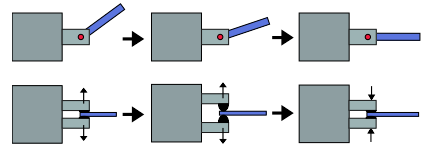
\includegraphics[scale=1.2]{chapter01/pics/1-1}
  \caption{在重力作用下旋转物体}
  \label{fig:1-1}
  \vspace{-0.3cm}
\end{figure}

在众多提高灵巧度的方法中,借助环境约束的方法显得更吸引眼球。
因为这种方法对传感需求低、控制算法简单,所以更具研究意义和实用价值。
在这个领域的研究中,N. Chavan-Dafle 等人将机器人手利用环境约束的
灵活程度定义为外部灵活度(Extrinsic dexterity),
他们认为实现这一灵活度需要通过以下三种运动:
外部接触驱动的准静态或准动态运动、利用重力的被动动态运动,
以及利用机械臂高速运动的主动动态运动\cite{ref7}。
本文主要研究的是第二类问题,这种方法只需要机器人手驱动器具有足够的精度和响应速度,
因此不需要使用复杂的控制和规划算法。
相比其他两种方法,被动动态运动的研究较少。
N.Chavan-Dafle、Alberto Rodriguez的团队设计的一个三指机器人手可以实现
不同物体的被动动态操作。
如将一个抓取的圆柱体在重力作用下滚动到手指上再滚动到手掌上,
或者将一个三棱柱从手上释放后,让它能立在桌面上\cite{ref7}(图\ref{fig:1-2})。
可以看出由于重力的作用形式单一,导致这种被动动态运动方式简单、应用范围不广,
主要是让物体在机械手的约束下依靠重力进行转动和下落,以此来实现手上操作。
不过这种方法也有它的优点,即操作过程中不需要同时控制机器人手和机械臂,
因此控制相对简单。

\begin{figure}[!ht]
  \centering
  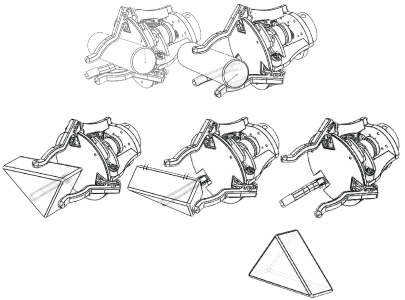
\includegraphics[scale=1]{chapter01/pics/1-2.png}
  \caption{两种被动动态运动}
  \label{fig:1-2}
  \vspace{-0.3cm}
\end{figure}

随着对手上操作方法研究的深入,快速响应机械手的需求慢慢增多,
特别是在动态运动过程分析中。在以往的研究中,
通常需要在执行操作任务时保持手指和操作对象之间的接触,
并且很少有人做机器人手的动态操作。
Noriatsu Furukaw 等人基于视觉反馈实现了快速的动态抓取。
如图\ref{fig:1-3}所示,他们利用一个高速机器人手将抓住的物体抛起,
然后在物体下落过程中机械臂调整到合适的姿态后抓取物体。
从实验结果来看,机器人手的抓取效果很好,
但是需要一个高速视觉伺服系统来提供视觉反馈\cite{ref8}。

\begin{figure}[!ht]
  \centering
  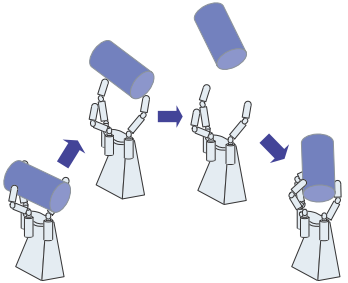
\includegraphics[scale=1]{chapter01/pics/1-3.png}
  \caption{机器人手进行动态操作}
  \label{fig:1-3}
  \vspace{-0.3cm}
\end{figure}

\section{研究现状分析}
目前国内对可利用环境约束的平行指夹具的研究较少,
国外的研究也大多还处于实验阶段,尚未投入实际生产中。
国外从纯运动学到基于统计学的运动规划研究都有涉及,
也有许多实验效果比较好的,但是研究数量较少。
特别是目前在这一领域大部分在研究外部驱动的准静态或准动态过程,
对于利用重力的被动动态过程研究少。
在理论知识方面,本项目的主要难点在于平行指夹具的结构设计和高速伺服电机的控制。
这些问题的研究已经比较成熟,所以本项目研究的理论基础是比较完备的。

\section{本文的主要研究内容}
本课题的研究内容主要是从运动过程中系统的物理学模型、对应的控制方法、
实验方案、仿真实验设计和具体实验操作等方面展开,
研究并验证单自由度机械手利用重力实现在手操作的实现方法。

